\documentclass[10pt]{beamer}

\usepackage{natbib}

\usetheme[progressbar=frametitle]{metropolis}
\usepackage{appendixnumberbeamer}

\usepackage{booktabs}
\usepackage[scale=2]{ccicons}

\usepackage{pgfplots}
\usepgfplotslibrary{dateplot}

\usepackage{xspace}
\newcommand{\themename}{\textbf{\textsc{metropolis}}\xspace}

\usepackage{amsmath, bm}
\usepackage[ruled,vlined]{algorithm2e}
\usepackage[utf8]{inputenc}


\title{Generative Adversarial Networks}
\subtitle{}
% \date{\today}
\date{}
\author{Davi Barreira}
\institute{FGV - Escola de Matemática Aplicada}
% \titlegraphic{\hfill\includegraphics[height=1.5cm]{logo.pdf}}
\usepackage{caption}
\captionsetup[figure]{font=footnotesize}

\begin{document}

\maketitle

\begin{frame}{Table of contents}
  \setbeamertemplate{section in toc}[sections numbered]
  \tableofcontents[hideallsubsections]
\end{frame}

\AtBeginSection{}
\section[Introdução]{Introdução}
\begin{frame}[fragile]{Introdução}

	\textbf{Generative Adversarial Networks} (GAN)
	foram originalmente introduzidas por \citet{goodfellow2014}.
	Essas redes são utilizadas com o objetivo de gerar
	dados sintéticos realísticos a partir de dados reais.

    \begin{figure}[H]
        \centering
        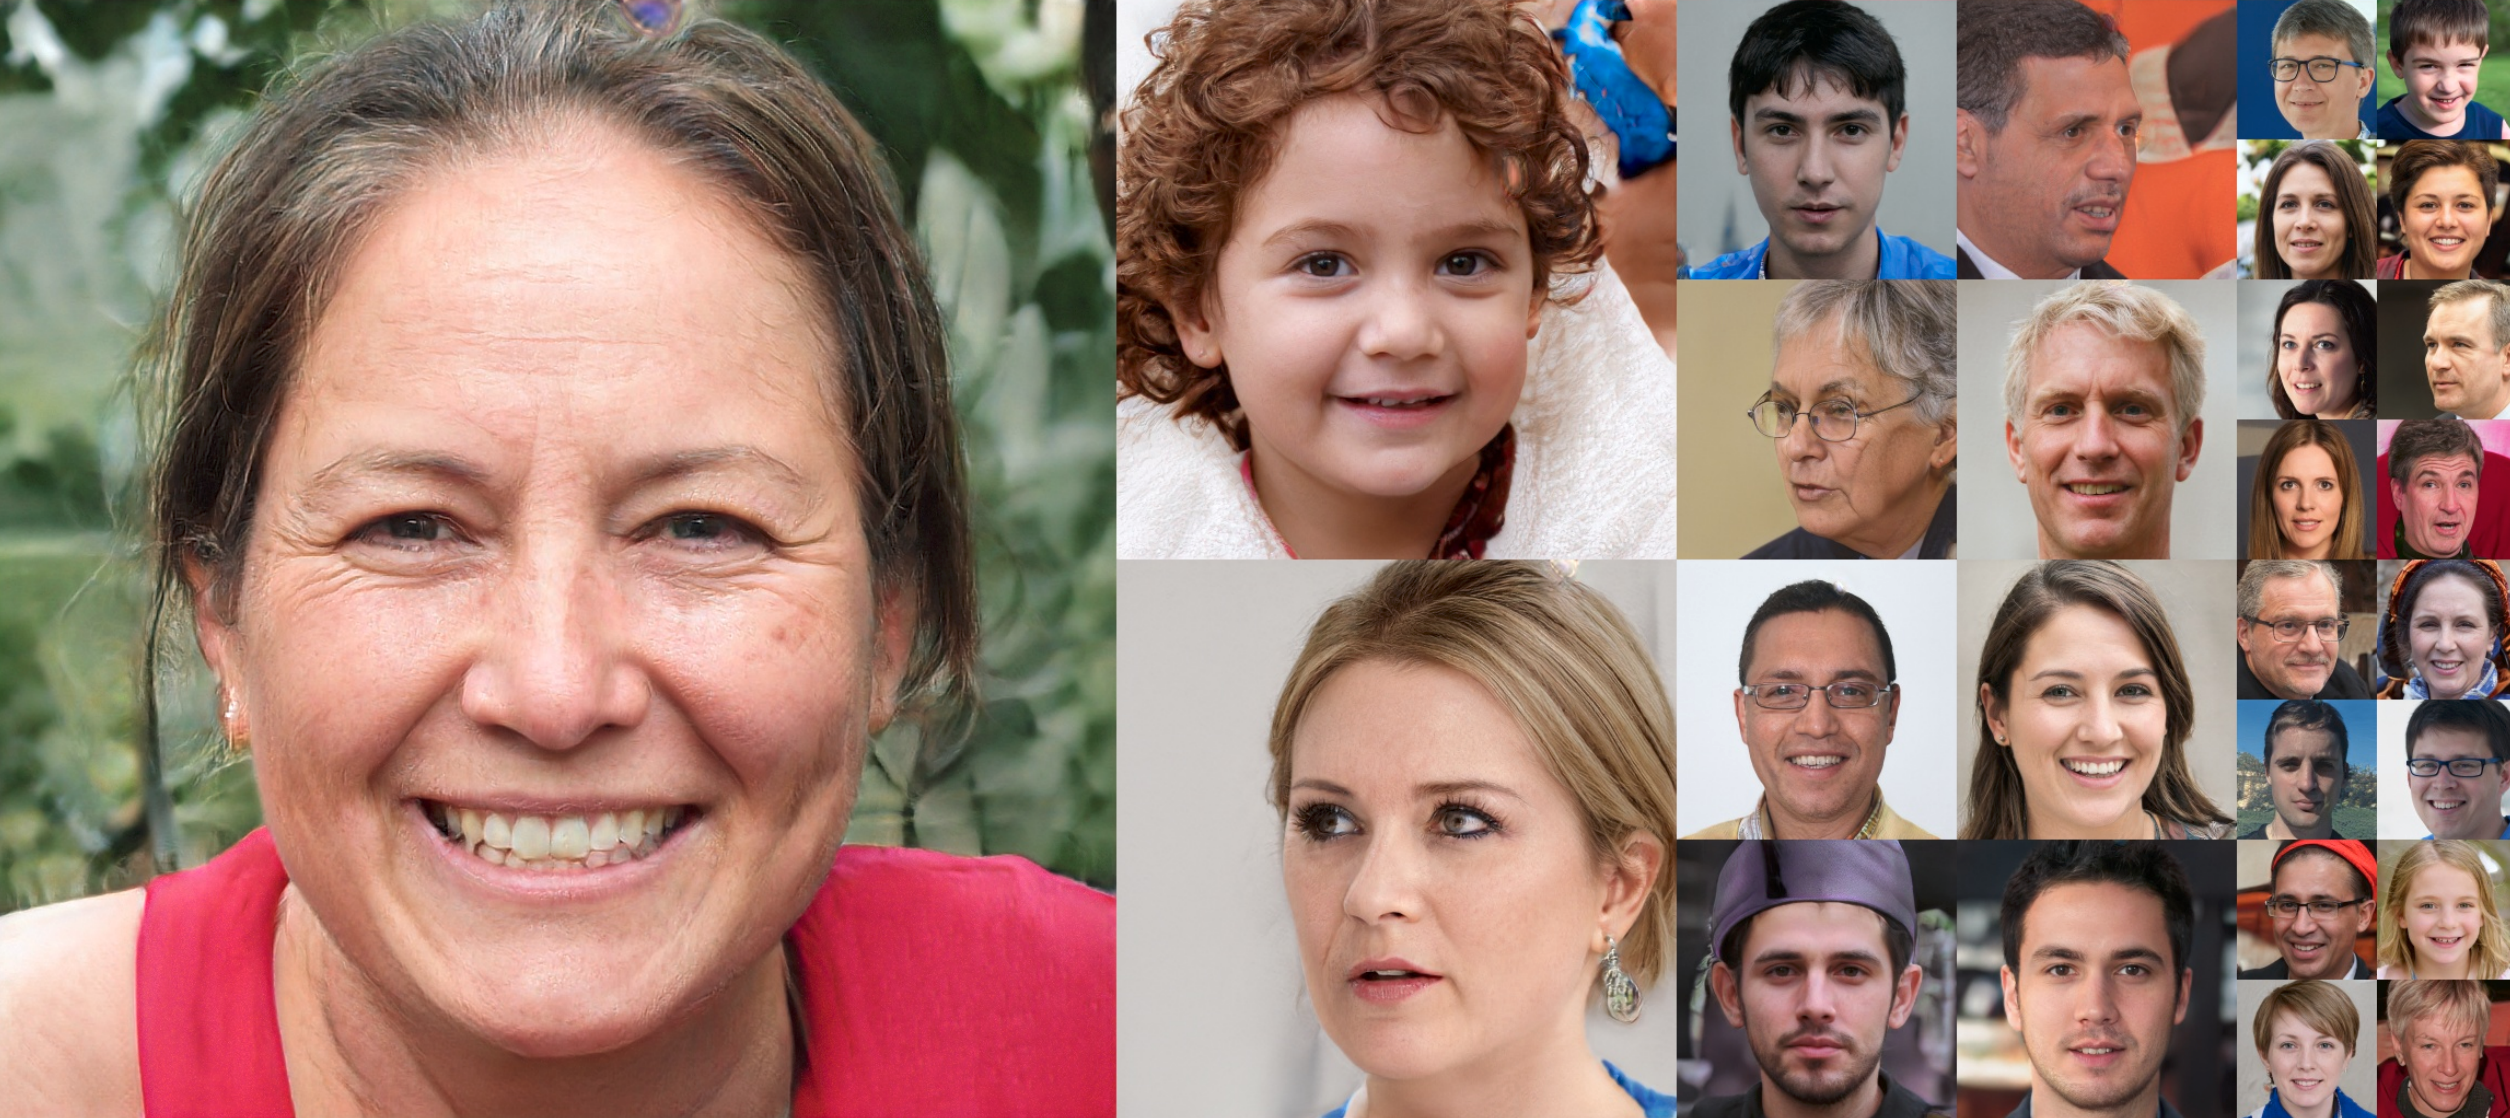
\includegraphics[width=6cm]{images/gans-faces.png}
        \caption{Faces geradas por GAN
        \footnote{https://towardsdatascience.com/generating-modern-arts-using-generative-adversarial-network-gan-on-spell-39f67f83c7b4}.}
    \end{figure}

\end{frame}

\begin{frame}[fragile]{Introdução}

	A geração de novas amostras sintéticas tem diferentes utilidades,
	como aprendizado semi-supervisionado, geração de exemplos
	adversariais, \textit{style transfer}, entre outros.

    \begin{figure}[H]
        \centering
        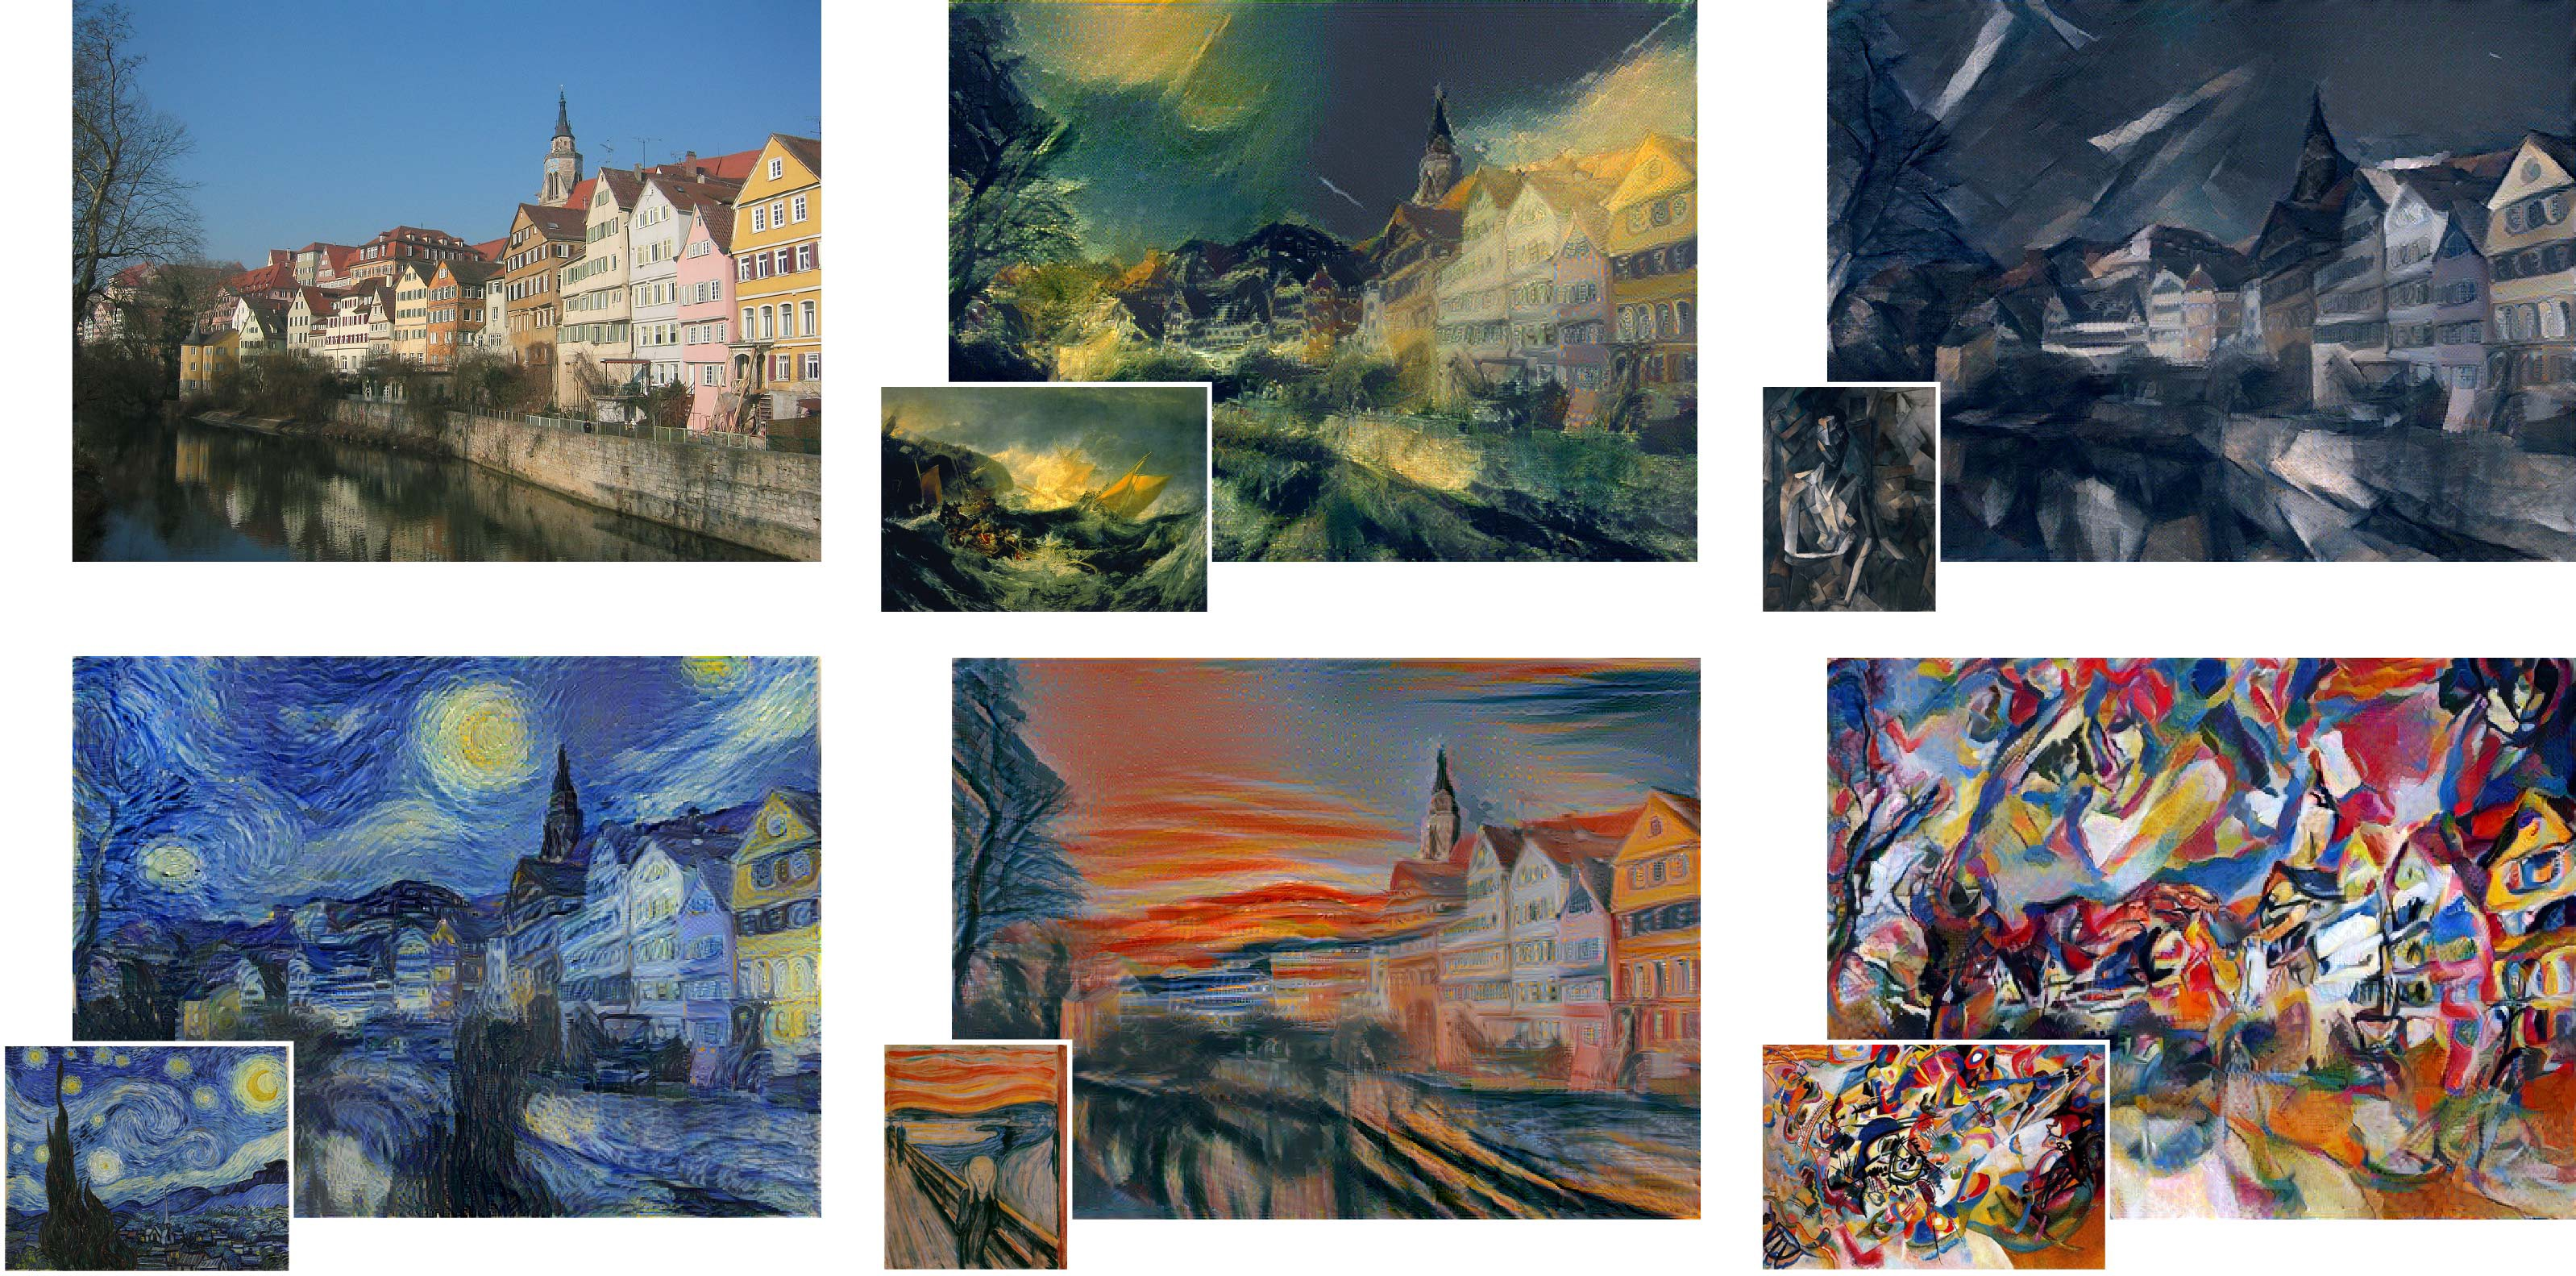
\includegraphics[width=6cm]{images/style-transfer.jpeg}
        \caption{Style transfer utilizando CycleGan
        \footnote{https://towardsdatascience.com/style-transfer-with-gans-on-hd-images-88e8efcf3716}.}
    \end{figure}


\end{frame}

\begin{frame}[fragile]{Introdução}

	A ideia geral por trás das GANs é utilizar duas redes neurais
	competindo uma com a outra, sendo uma rede responsável por
	gerar amostras parecidas com os dados reais, enquanto a outra
	busca identificar quando o dado é real ou sintético.

    \begin{figure}[H]
        \centering
        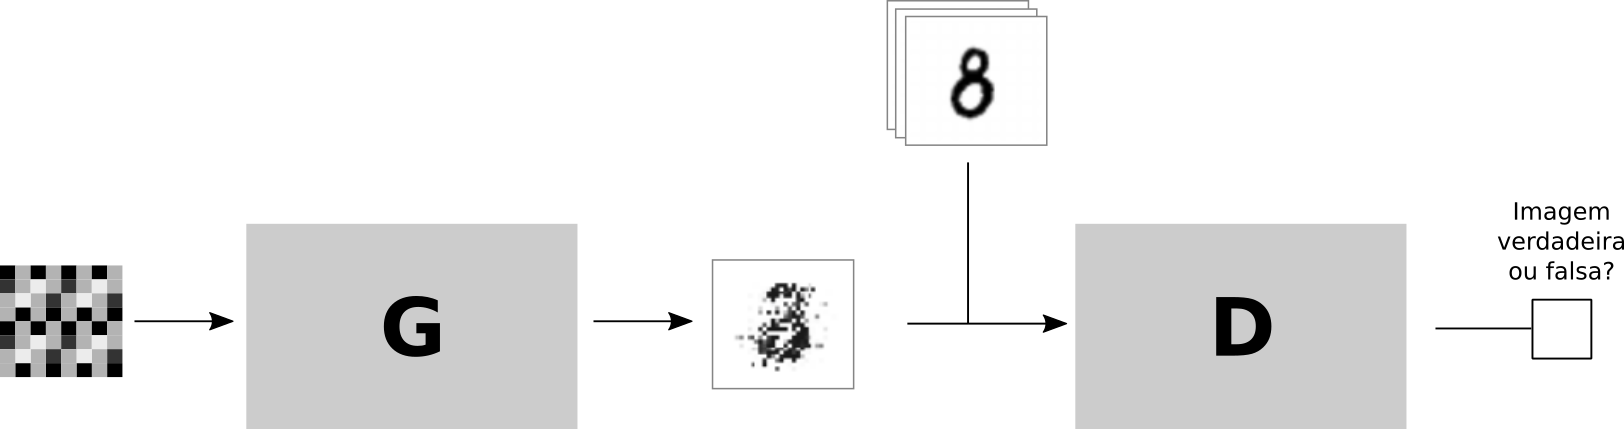
\includegraphics[width=10cm]{images/gan_scheme.png}
        \caption{Desenho esquemático de uma GAN "convencional".}
    \end{figure}


\end{frame}


\AtBeginSection{}
\section[Teoria]{Formalização Teórica}
\begin{frame}[fragile]{Formalização Teórica}

  \footnotesize
  \begin{algorithm}[H]
  \SetAlgoLined
  \For{número de iterações de treino}{
  	\For{k passos}{
  		Amostre $m$ valores $\{\bm z^{(1)},...,\bm z^{(m)} \}$
  		da priori $p_z(\bm z)$;

  		Amostre $m$ exemplos $\{\bm x^{(1)},...,\bm x^{(m)} \}$
  		da fução dos dados $p_{data}(\bm x)$;

  		Atualize o \textit{discriminator} utilizando
  		\textit{stochastic gradient descent}:
  		$$
  		\nabla_{\theta_d}\frac{1}{m}\sum^{m}_{i=1}
  		\left[
  		log D(\bm x^{(i)}) + log(1-D(G(\bm z^{(i)})))
  		\right]
  		$$
  	}

	Amostre $m$ valores $\{\bm z^{(1)},...,\bm z^{(m)} \}$
	da priori $p_z(\bm z)$;

	Atualize o \textit{generator} utilizando
	\textit{stochastic gradient descent}:
  		$$
  		\nabla_{\theta_d}\frac{1}{m}\sum^{m}_{i=1}
  		log(1-D(G(\bm z^{(i)})))
  		$$
  }
   \caption{GAN descrita em \citet{goodfellow2014}}
  \end{algorithm}

\end{frame}

\begin{frame}[allowframebreaks]{References}

% \renewcommand{\bibsection}{\section{}}
  \renewcommand{\section}[2]{}%
  \bibliography{gan}
  % \bibliographystyle{plainnat}
  % \bibliographystyle{plain}
  % \bibliographystyle{abbrv}
  \bibliographystyle{apa}

\end{frame}

\end{document}
